\chapter{Réalisations}
\label{Developpement}


\section{Les Projets}

\subsection{MobiSaaS}

\subsubsection{Présentation}

Le projet "MobiSaaS" s'inscrit dans la démarche d'entreprise de proposer des solutions en mode \textbf{SAAS}. Le projet consiste d'une manière générale à exposer les fonctionnalités de la solution desktop du produit "MobiAnalyst"(Fig. \ref{OffreMobiAnalyst}).

Mon stage et les développements demandées concernent la brique ou le composant "MobiAdmin". Dans l'objectif de gérer les données du client, je dois proposer un service de gestion des données de transport dans l’espace privatif du client.
La fonctionnalité à développer est = "Upload de données GTFS (fichier au format zip)".\\ 
Un jeu de données GTFS (ensemble de fichiers .txt) peut en contenir un seul ou plusieurs. Il faudra récupérer et renseigner les metadonnées de chaque upload de fichier :
\begin{itemize}
\item Nom 
\item Date d’upload ou de la version du GTFS
\item Licence (open data/ restreint/ privé)
\item Url si open data
\item Commentaire libre
\item Chemin vers la données
\end{itemsize}

\begin{figure}[!h]
\centering
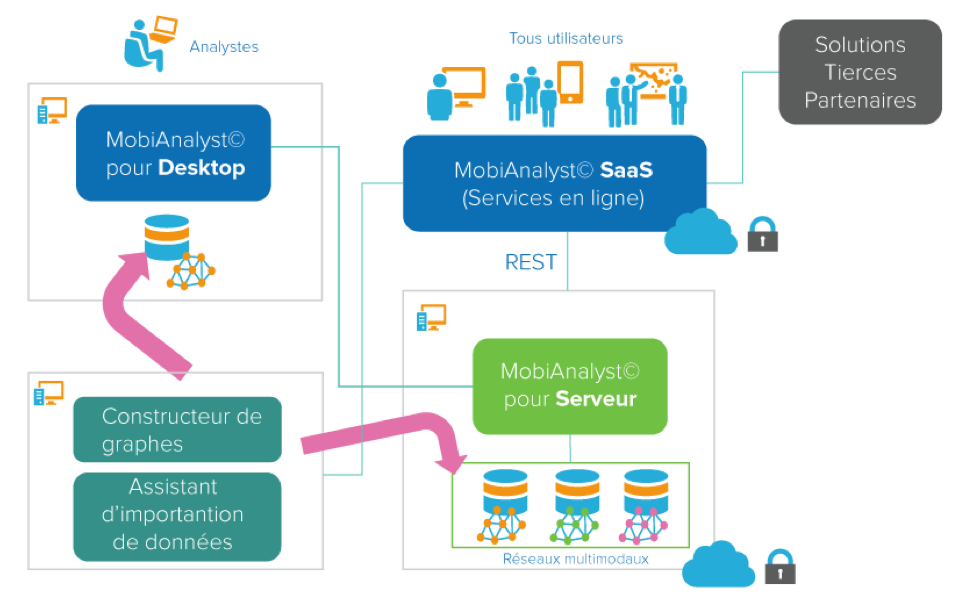
\includegraphics[width=14cm]{images/offre_MobiAnalyst.png}
\caption{\label{OffreMobiAnalyst}Offre du produit MobiAnalyst}
\end{figure} 

\subsubsection{Eléments de spécifications fonctionnelles et techniques}

\paragraph{Architecture actuelle}

La figure \ref{fig:architecture} détaille l'ensemble des briques logicielles nécessaires au fonctionnement de la plate-forme
MobiAnalyst as a Service (MobiSAAS) :
\begin{itemize}
\item \textbf{AGS} : ArcGIS Server. Le serveur de Système d'Information Géographique (SIG) permettant de publier et d'administrer des services cartographiques (MapService).
      Dans notre cas, les MapServices déployés sont des réseaux routiers et de transport en commun (TC),
			accompagnés de tables horaires (TimeTable) contenant les horaires
			des TC.
\item \textbf{SOE}: Server Object Extension. Nous utilisons le mécanisme d'extension SOE pour déployer sur un MapService un service spécifique à MobiSAAS. Un SOE est
      une fonctionnalité qui se déploie sur un MapService et qui expose en Web Service (REST ou SOAP) les solveurs de MobiAnalyst.
\item \textbf{MobiAdmin}: Serveur REST d'administration MobiSAAS. Ce serveur (basé sur Java) est le point d'entrée des utilisateurs des services REST de MoniAnalyst.
      Il redirige les requêtes métiers vers le bon SOE déployé, il trace ces requêtes et enrichit la base de données client de MobiAnalyst.
			L'authentification qui est faite dans les requêtes utilise les comptes d'AGS créés au préalable.
\item \textbf{Postgres} : Système de gestion de base de données. Cette base contient les données clients de MobiAnalyst : profil, traces d'utilisation de MobiSAAS.
\item \textbf{MongoDB} : Système de gestion de base de données. Cette base contient les logs (statistiques mesurées en temps réel) correspondant aux services REST de MobiSAAS
\end{itemize}

\begin{figure}[h]
	\centering
		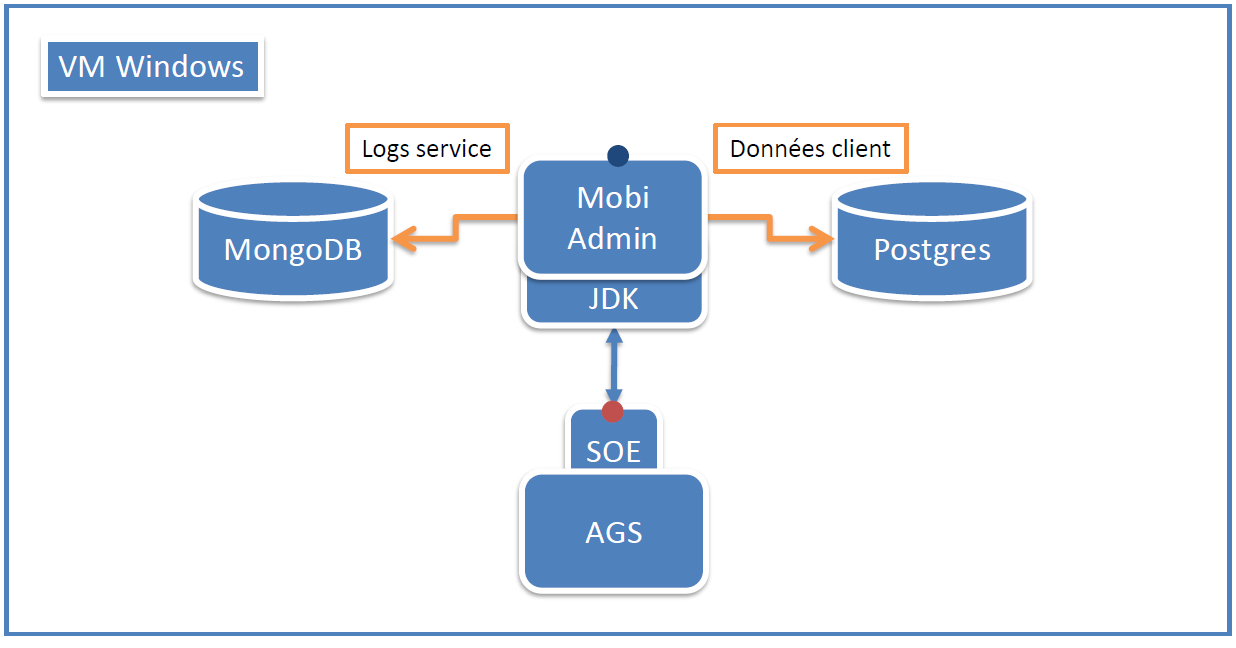
\includegraphics[width=0.8\textwidth]{images/architecture.png}
	\caption{Architecture globale.}
	\label{fig:architecture}
\end{figure}

Pour le composant "MobiAdmin" le choix technologique majeur est d'utiliser le framework DropWizard (cf. Annexe \ref{Annexe B}). Ce framework orienté micro-services nous permet de fournir notamment un serveur embarqué HTTP "Jetty". Jersey pour la partie webservice REST qui est l'implémentation de référence de la spécification JAX-RS. Ou encore Jakson pour la dé/sérialisation du JSON.\\


\subsubsection{Développements}

Le but de mon stage est de développer des web services WS en amont du DataWizard en mode \textbf{SAAS} (cf.définition) dont principalement l'import de données GTFS. L'objectif de ce service est de pouvoir manipuler ces données (comme le fait le DataWizard) et ainsi pouvoir récupérer des métadonnées ex: l'extension géographique des données, le nom de l'agence, le nombre de lignes, le mode de transport,...\\

L'environnement de développement est donc un projet Java EE Maven composé des éléments de Dropwizard. \\
Ces WS sont à priori “lourds”, sachant qu'un jeu de données (ex: GTFS\footnote{\url{https://developers.google.com/transit/gtfs/reference}}) fait plusieurs centaines de Mo, les opérations de téléchargement, validation, traitement, stockage dans en base,... vont être long à renvoyer une réponse au client après chaque requête. Les WS à développer sont donc asynchrones. De plus, une contrainte supplémentaire et que le service doit supporter plusieurs requêtes simultanées, il faudra donc s'orienter vers un développement en mode "programmation concurrente".\\


\subsubsection{Résultats obtenus / Difficultés rencontrées}

J'ai tout d'abord commencé par découvrir Maven (cf. Annexe \ref{Annexe A}), les projets, les modules, le désormais célèbre fichier \textbf{POM}, etc...
Ensuite, je me suis documenté sur le code métier existant, et chercher des outils ou librairies de professionnels du domaine (cf. Outils métiers \ref{OBA}).
Enfin, après le "Getting Started" de Dropwizard\footnote{\url{https://dropwizard.github.io/dropwizard/getting-started.html}}, une fois tout cela bien maîtrisé, j'ai pu  commencé la conception et le développement de services web REST.\\

J'ai choisit de stocker les informations concernant ma partie de l'application dans une table PostgreSQL (Fig \ref{TablePostgres})\\
\begin{figure}[!h]
\centering
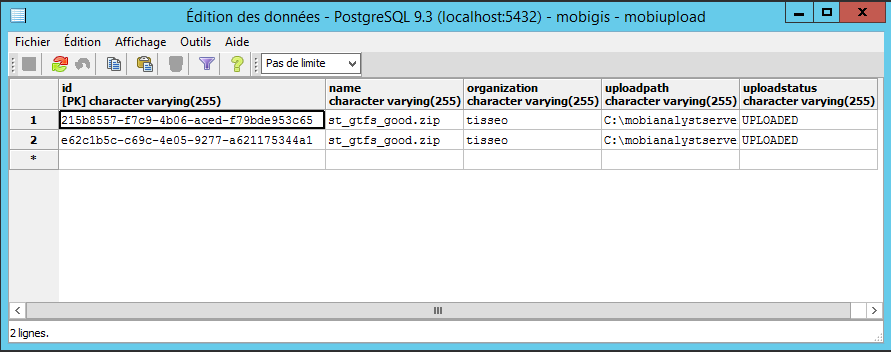
\includegraphics[width=14cm]{images/tablePostgres_mobiupload_small.png}
\caption{\label{TablePostgres}Table des uploads sur le SGBD PostgreSQL}
\end{figure} 

A chaque requête POST du client, je créé une instance d'objet Upload, je saisis les informations dans ma table de suivi, et je stocke les données envoyées sur le serveur. Pour chaque client ou utilisateur, pour chaque type de données, il y a un répertoire personnalisé, chaque upload est "taggé" d'un identifiant unique "UUID".
Le code métier qui a été implémenté est pour le moment le test sur le type de données envoyées, la validation des données et la production d'un rapport d'un validation (JSON), enfin l'extraction (récursive) des données contenues dans l'archive.\\

\subsubsection{Perspectives}

L'idéal d'un programme développé dans un langage orienté objet, est la généricité, et la réutilisation d'un maximum de composants. Dans ce travail, l'objectif est clairement de produire un maximum de composant abstrait et de méthodes réutilisables. Les perspectives du projet "MobiSaaS" sont nombreuses : gérer une architecture distribuée, augmenter les fonctionnalités SaaS notamment les principales du projet "DataWizard".\\

\subsection{DataWizard}

\subsubsection{Présentation}

Le projet "DataWizard", ensemble de scrips Python et SQL c'est une application dont le but est d'ingérer des données de transports, et de voirie dans une base de données spatiales (PostgreSQL/PostGIS \ref{Postgis}) afin de produire en sortie un réseau de transport (Network Dataset ou NDS).\\


\subsubsection{Eléments de spécifications fonctionnelles et techniques}

Afin de fournir, un réseau conforme aux attentes du logiciel MobiAnalyst et des experts en analyse de réseaux de transports, l'équipe me fournit une spécification de métadonnées à extraire des données en entrée du DataWizard (\ref{DW_Metadata}).\\

\begin{figure}[!h]
\centering
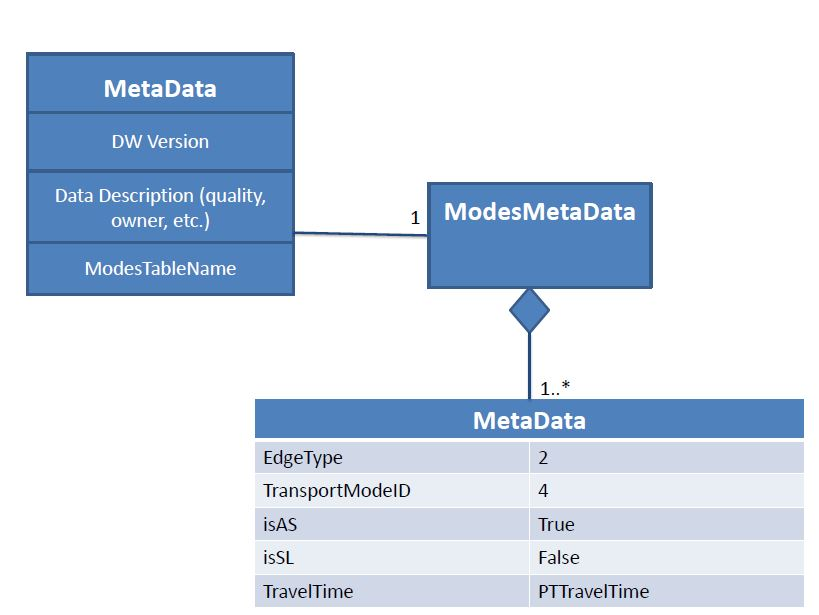
\includegraphics[width=14cm]{images/DW_specMetadata.JPG}
\caption{\label{DW_Metadata}Schéma des tables de métadonnées}
\end{figure} 

\subsubsection{Développements}

J'intègre tout d'abord le projet en tant qu'utilisateur, j'exploite des données et produits des réseaux (Bordeaux, Champagne-Ardennes, Montreal, Melbourne,etc...) Ensuite, petit à petit je suis le plan de charge issu du projet Redmine et corrige des bugs, et anomalies.\\


\subsubsection{Résultats obtenus / Difficultés rencontrées}

Les données sont complexes, GTFS ou voirie (Données Here ou OpenStreetMap). La base de données "DataWizard" possède de nombreux schémas, et les requêtes SQL sont parfois très complexes mêlant fonctions, et requêtes géographiques.\\


\subsubsection{Perspectives}

